\documentclass{article}
\usepackage{acronym}
\usepackage{hyperref}
\usepackage{geometry}
\usepackage{graphicx}

\usepackage{listings}
\lstset{
    breaklines=true,
    basicstyle=\ttfamily
}

\geometry{
    a4paper,
    total={170mm,257mm},
    left=20mm,
    top=20mm,
}

\begin{document}
\author{
    Team SwAG
}


\title{Travel w/ SwAG}
\maketitle

\begin{acronym}
\acro{SwAG}{\textbf{S}oft\textbf{w}are \textbf{A}gents doing \textbf{G}reat things}
\end{acronym}


Travel w/ SwAG is an assistant developed by the \ac{SwAG} team. The assistant is designed to be a personalized travel assistant that can currently help with the following:

\begin{itemize}
\item Understanding \& navigating your current surroundings.
\item Finding things to do and places to eat.
\item Identifying landmarks, monuments, and other points of interest.
\item Describing art, statues, and other visual elements.
\end{itemize}

    The assistant is built on top of the Anthropic API, along with a series of tools that it can use to obtain the information it requires. It has a unique feature in that it uses SAM (Segment Anything Model\footnote{\url{https://ai.meta.com/sam2/}}) to segment images, allowing for a more interactive experience. The target audience for this is basically anyone, but is aimed towards tourists or people who are new to an area. The goal is to save time and get more out of your trip, in both information and experience.

The users can interact with the assistant via text or images, and the assistant will respond with the information that it has found. We have also included a demo video, which shows the assistant in action, which you can watch here: \url{https://www.youtube.com/watch?v=41-gEmVGCjk}

\section{Why Travel w/ SwAG?}

We wanted to create a travel assistant that was more interactive and could provide a more personalized experience. We felt that there was a gap in the market with current travel assistants as they are either bad or just advertisements\footnote{This is an opinion and not a fact}. Traditional travel apps often overwhelm users with generic information or are filled with sponsored content, making it difficult to find authentic, relevant experiences. We wanted to build an application that helps users on 'the ground', providing insights and overall enhancing their travel experience.

Travel w/ SwAG is therefore a multi-modal personalized assistant that sits in your pocket and can help you navigate a place with 'SwAG'. It can understand your intentions, where you are and what you're looking at to provide you with the information they need.

\section{Features}

Travel w/ SwAG  offers two powerful, interactive features:

\begin{itemize}
\item \textbf{SwAG Assistant}: This is a text-based assistant for trip planning \& navigation. It utilises a variety of tools including route optimization tools \& interactions with the Google Maps API, all handled by Claude Sonnet 3.5
\item \textbf{Everywhere TourGuide}: This is a vision-based assistant that analyses images taken at the users current location to determine what they are looking at, and then provide information on it. This also utilises a number of tools, including a internet search tool carried out by the JinaAI engine\footnote{\url{https://jina.ai/}}.
\end{itemize}

The implementation leverages Anthropic's tool use feature. We clearly defined the set of tools with Pydantic models for maintainability and usability. These can be easily translated to the format required by Anthropic for the tool use feature.

Both the features are wrappers around the same assistant class, however have different tools \& prompts. This is where in the future we would like to merge this into 1 assistant, with custom query routing \& tool retrieval based on the user's query.

\subsection{SwAG Assistant}

One interesting feature of this assistant is to help to plan trips. An example we used in the provided video was:

\begin{lstlisting}
I want to plan a trip to Marseille to eat Tajine, hike to Mont Blanc, and visit Barcelona. What's the total road trip distance, and how far will I hike on foot? Can you help me plan an itinerary?
\end{lstlisting}

The assistant will then research all the information that it needs, including:

\begin{itemize}
\item Searching the internet for the lat/lng of the locations (Using JinaAI)
\item Calculating the distance between the locations (Using Google Maps API)
\item Optimizing the route (Using custom route optimization tools)
\end{itemize}

This will return a detailed plan back to user, including the total distance, the distances they can hike, and a detailed itinerary. From that, the user can further interact with the assistant, for example by asking about specific Morrocan restaurants in Marseille near their hotel.

The assistant is able to understand the user's intentions and provide them with the information they need, in a way that is easy to understand and interact with.

\subsection{Everywhere TourGuide}

The TourGuide is a vision-based assistant that acts as a friendly 'tourguide' for any situation the user might be in. It analyses an image taken at the users current location to figure out what they are looking at, and then provides information on it.

The feature which makes this tool unique is the built in object segmentation using SAMv2. SAM is a model built by Meta that can segment images based on a series of clicks. This means the user can 'click' on specific element of the image, for example the hand of a statue or a specific symbol within a painting. If that element has a unique story behind, the assistant will provide that story to the user.

In the provided video, we used the example of the Trevi Fountain in Rome, masking (segmenting with a fill) one of the statues in the right-most niche. In this case, it was the statue of Health, which the assistant was able to correctly identify. See Fig. \ref{fig:mask} for an example of the output of SAM. For this we are using the SAMv2 Tiny model, which is a smaller version of the full SAMv2 model, but still provides accurate results.

\begin{figure}
    \centering
    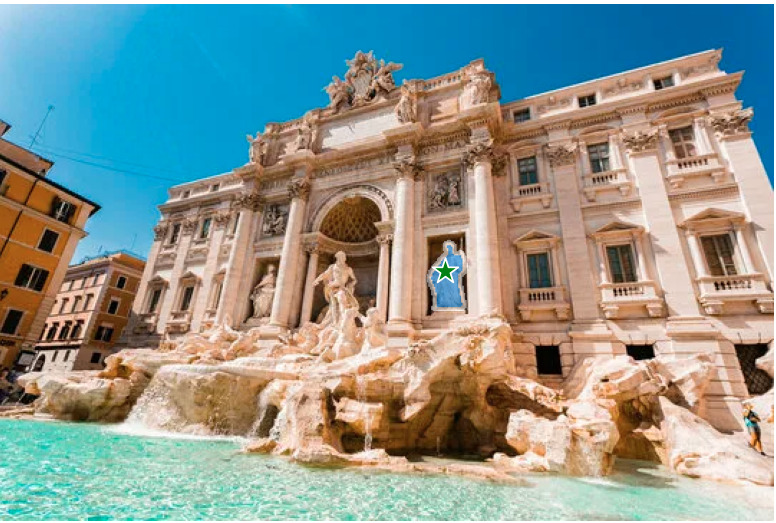
\includegraphics[width=0.5\textwidth]{../imgs/masked_tf.png}
    \caption{Example of SAMv2 Tiny output on the Trevi Fountain}
    \label{fig:mask}
\end{figure}

\section{Future Work}

We have a number of ideas for future work, including:

\begin{itemize}
\item \textbf{Integration with VR/AR}: We believe that the assistant could be even more useful it it was integrated with VR/AR, utilising pose-detection to auto-invoke the SAM (via pointing) and therefore the tourguide.
\item \textbf{TTS/STT}: We would like to integrate text-to-speech and speech-to-text capabilities, to make the assistant more accessible, in both the fact that you wouldn't need to take out your phone but also allowing visually impaired users to make use of the application
\item \textbf{Memory}: Tying in with the theme of making the assistant more personalized, we would like to add a memory feature, where the assistant can remember previous interactions with the user and use that to provide more personalized responses.
\end{itemize}

\section{Conclusion}

Travel w/ SwAG represents a step forward in personalized travel assistance, combining modern AI capabilities with practical tools for travellers. By leveraging technologies like Claude Sonnet 3.5, SAMv2, and various APIs, we've created an assistant that can truly understand and respond to users' needs in real-time. Whether planning complex itineraries or exploring new locations, Travel w/ SwAG aims to enhance the travel experience through intelligent, interactive assistance.

We thank Anthropic for providing access to their API, and the JinaAI team for their search capabilities that made this project possible.

\end{document}
